\documentclass[main.tex]{subfiles}

\begin{document}
	
	El laboratorio realizado tiene como principales objetivos los siguientes:
	
	\begin{itemize}
		\item Consolidar los conceptos de teoría moderna mediante la implementación circuital.
		\item Simular e implementar el filtro con componentes activos de precisión.
		\item Medir las partes de la función transferencia para frecuencias menores a 100 kHz.
	\end{itemize}
	
	Para realizarlo, se selecciono la siguiente plantilla de filtrado:
	
	\bigskip
	
	\centering
	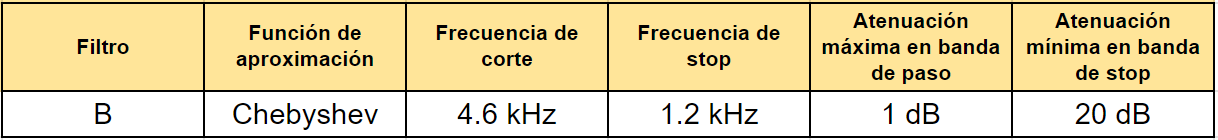
\includegraphics[width=15cm]{./../Imagenes/PlantillaConsigna.png}
	\raggedright
		
	
\end{document}